\documentclass[a4paper,11pt,fleqn]{article}%fleqn pour aligner les equations à gauche
\usepackage{../../Styles/Cours}

\newcommand{\chnum}{Chapitre 16}
\newcommand{\chtitle}{Bilan radiatif de la Terre}
\newcommand{\dtype}{Activité}

\begin{document}
	\maketitle
	
	Les experts du Groupe intergouvernemental d'experts sur l'évolution du climat (GIEC) prévoient, à l'horizon 2100, une augmentation moyenne des températures de \SI{3}{\celsius} à \SI{4}{\celsius} sur la surface terrestre. Les conséquences seraient, entre autres, une élévation du niveau des mers et des océans de plus d'un mètre, et une perte considérable d'étendues terrestres pour les régions côtières ou à faible altitude.\\
	\textbf{Quels modèles permettent d'estimer l'évolution de la température à la surface de la Terre?}
\begin{figure}[h!]
	\begin{minipage}{.48\linewidth}
		\caption{Prévision du GIEC d'ici 2100}
		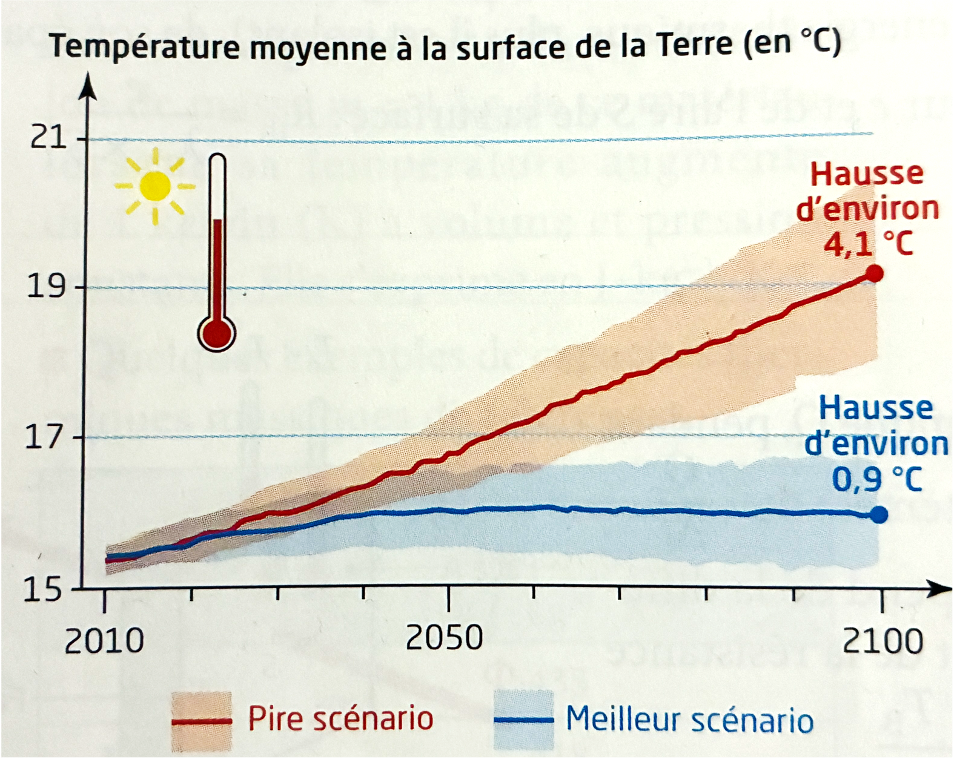
\includegraphics[width=\linewidth]{Ressources/TSPE_C16_AE3_Fig1.png}
	\end{minipage}
	\begin{minipage}{.48\linewidth}
		\caption{Corps noir}
		Un corps noir est un objet théorique qui absorbe intégralement le rayonnement électromagnétique qu'il reçoit.\\
		Sous l'effet de l'agitation thermique induite, ce corps émet alors un rayonnement électromagnétique qui ne dépend que de sa température. La loi de Stefan-Boltzmann permet de relier cette température $T$ au flux thermique surfacique rayonné $\varphi_E$ :
		\begin{tabular}{c|m{.7\linewidth}}
			\multirow{3}{*}{$\varphi_E = \sigma \cdot T^4$} & $\varphi_E$ en watt par mètre carré (\unit{\watt\per\meter\squared})\\
			&$\sigma$  constante de Stefan-Boltzmann, $\sigma  = \SI{5,67E-8} {\watt\per\meter\squared\per\kelvin\tothe{4}}$\\
			&$T$ en kelvin (\unit{\kelvin})\\
		\end{tabular}
	\end{minipage}
\end{figure}
\begin{figure}[h!]
	\caption{Albédo}
	\begin{minipage}{.68\linewidth}
		Considérons un système qui reçoit un rayonnement électromagnétique bien déterminé, par exemple le rayonnement solaire. Une partie du rayonnement solaire reçu est réfléchi et diffusé, et une autre partie est absorbée par le système.\\
		L'albédo A est le quotient du flux thermique surfacique $\varphi_D$ réfléchi et diffusé par ce système par le flux thermique surfacique $\varphi_S$ incident : $A = \dfrac{\varphi_D}{\varphi_S}$.\\
		Le flux thermique surfacique moyen émis par le Soleil et reçu par le système \{Terre; atmosphère\} est égal
		à : $\varphi_S = \SI{350} {\watt\per\meter\squared}$.\\
		Les albédos de différentes surfaces sont donnés dans le tableau ci-contre.\\
		Le système \{Terre; atmosphère\} présente un albédo moyen considérable (de l'ordre de 0,3), auquel les conti-nents, le sable et la neige apportent une contribution très importante.
	\end{minipage} 
	\begin{minipage}{.3\linewidth}
		\begin{tabular}{|c|c|}
			\hline
			\textbf{Typer de surface} & \textbf{Albédo}\\
			\hline
			Mer & \num{0,1}\\
			\hline
			Forêt & \num{0,1}\\
			\hline
			Nuage & \num{0,5} à \num{0,8}\\
			\hline
			Glace & \num{0,5} à \num{0,7}\\
			\hline
			Neige fraîche & \num{0,8}\\
			\hline
		\end{tabular}
	\end{minipage}
\end{figure}

\begin{figure}[h!]
	\caption{Influence de l'atmosphère}
	Une atmosphère contenant des gaz à effet de serre (eau, dioxyde de carbone, méthane, ozone, etc.) absorbe une proportion a du rayonnement emis par la planète. Cette proportion est d'environ \SI{75}{\percent} pour la Terre. Elle dépend des concentrations des gaz à effet de serre. Plus ces concentrations sont grandes, plus l'absorption, et donc la valeur de $\alpha$, sont importantes.\\
	Ce rayonnement absorbé est ensuite ré-émis aléatoirement dans toutes les directions. Ainsi, environ la moitié du rayonnement infrarouge absorbé par les gaz. à effet de serre repart dans l'espace, tandis que l'autre moitié retourne à la surface terrestre.
\end{figure}

\begin{figure}[h!]
	\caption{Différents modèles possibles}
	Pour chacun des modèles proposés, le système {Terre; atmosphère} est considéré en équilibre radiatif : il reçoit au total un flux thermique moyen égal à celui qu'il réémet dans l'espace. La température moyenne de surface de la Terre est alors constante.
	Le rayonnement émis par la Terre est supposé semblable à celui d'un corps noir.\\
	\begin{center}
		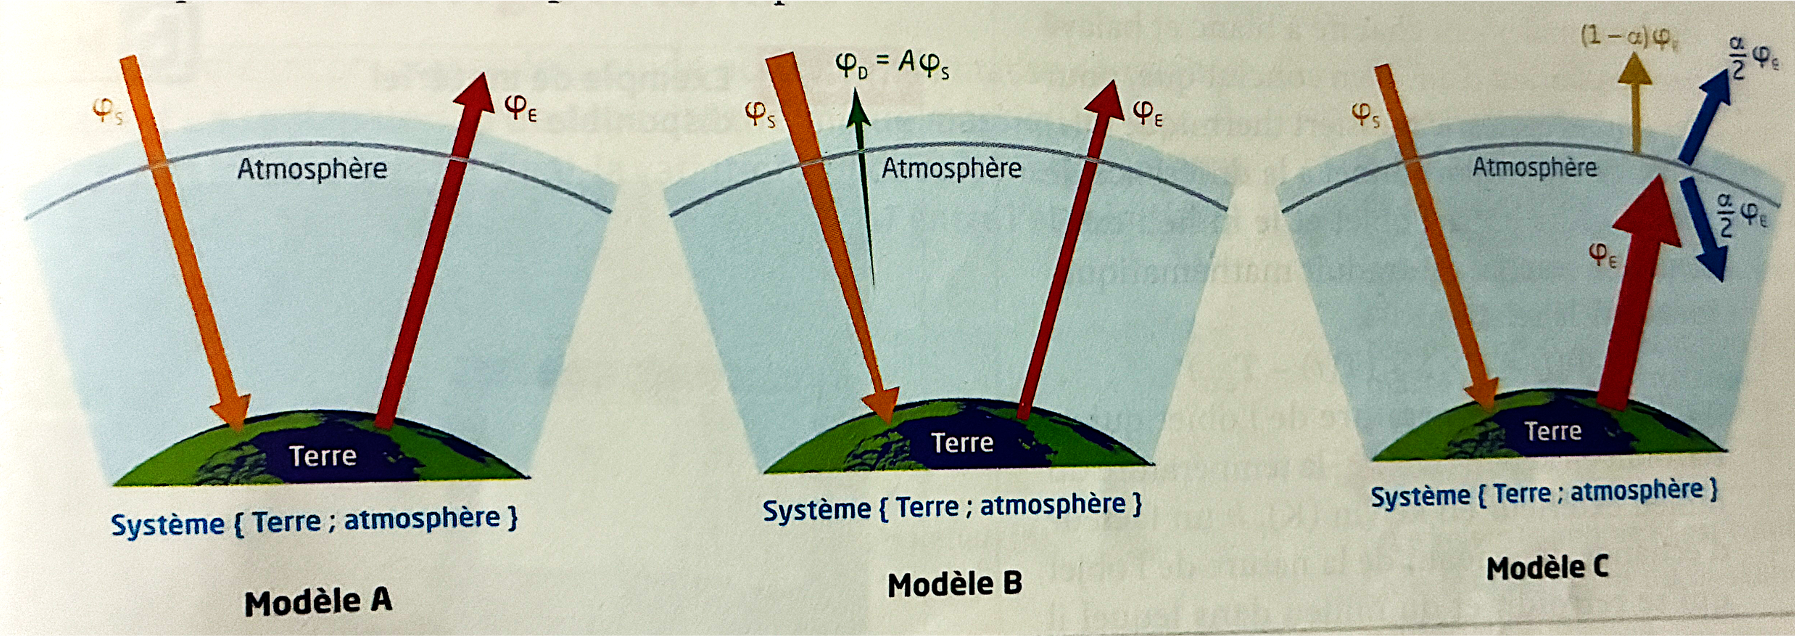
\includegraphics[width=.8\linewidth]{Ressources/TSPE_C16_AE3_Fig2.png}
	\end{center}
\end{figure}

\begin{figure}[h!]
	\caption*{Questions :}
	\begin{enumerate}
		\item Associer chacun des modèles présentés dans le DOC.5 au(x) DOC. 2, 3 et 4 correspondant(s).
		\item  Dans le cadre du modèle \textbf{A} : 
		\begin{itemize}
			\item utiliser la condition d'équilibre radiatif décrite dans le DOC. 5 pour déterminer la valeur du flux thermique surfacique $\varphi_E$ de rayonné par la surface terrestre
			\item en déduire la valeur de la température moyenne $T_{T,A}$ de la surface terrestre estimée dans le cadre du modèle \textbf{A} puis commenter le résultat obtenu.
		\end{itemize}
		\item Dans le cadre du modèle \textbf{B} ou du modèle \textbf{C} :
		\begin{itemize}
			\item utiliser la condition d'équilibre radiatif décrite dans le DOC. 5 pour établir la relation entre le flux thermique surfacique reçu du Soleil $\varphi_S$, le flux thermique surfacique rayonné $\varphi_E$ par la surface terrestre et l'albédo terrestre A (pour le modèle \textbf{B}) ou la proportion $\alpha$ du flux thermique surfacique rayonné par la surface terrestre et absorbé par l'atmosphère (pour le modèle \textbf{C});
			\item en déduire la valeur de la température moyenne de la surface terrestre $T_{T,B}$, ou $T_{T,C}$ estimée dans le cadre du modèle étudié puis commenter le résultat obtenu.
		\end{itemize}
		\item Présenter oralement le modèle étudié (\textbf{B} ou \textbf{C}) et les résultats obtenus aux élèves qui ont traité l'autre modèle.
		\item Montrer qu'un quatrième modèle, tenant compte à la fois de l'albédo et de l'effet de serre, permet d'obtenir l'expression suivante de la température moyenne de la surface terrestre : $$T_{T,D} = \left( \dfrac{2\times (1-A)}{(2-\alpha)\times \sigma}\cdot \varphi_S\right)^{\frac{1}{4}}$$
		Calculer $T_{T,D}$ et conclure.
		\item En se basant sur ce quatrième modèle et sur ses résultats, commenter l'influence de l'effet de serre et de l'albédo sur la température moyenne de la surface terrestre.
	\end{enumerate}
\end{figure}

\end{document}